\documentclass[conference]{IEEEtran}

% --- Preamble ---
\usepackage[utf8]{inputenc}
\usepackage[T1]{fontenc}
\usepackage{amsmath,amssymb}
\usepackage{graphicx}
\graphicspath{{figs/}} % <-- 図の既定パス
\usepackage{cite}
\usepackage{url}
\usepackage{hyperref}

% TikZ(座標計算に calc を追加)
\usepackage{tikz}
\usetikzlibrary{arrows.meta,positioning,fit,calc,shapes.misc}

\title{Time-Response-Aware Design of CFET Interconnect Delay, Self-Heating, and Stress Coupling via PID+FSM+LLM Supervision}

\author{
  \IEEEauthorblockN{Shinichi Samizo}
  \IEEEauthorblockA{Independent Semiconductor Researcher\\
  Project Design Hub, Samizo-AITL\\
  \textit{Email:} \href{mailto:shin3t72@gmail.com}{shin3t72@gmail.com}\quad
  \textit{GitHub:} \href{https://github.com/Samizo-AITL}{Samizo-AITL}}
}

\begin{document}
\maketitle

\begin{abstract}
Gate-all-around (GAA) nanosheet FETs can be designed under static assumptions, where parasitics and thermal effects are treated as fixed values. However, complementary FETs (CFETs) with stacked n/p channels suffer from strong vertical self-heating and stress coupling. These effects vary dynamically, leading to RC delay shifts that static design cannot capture. This paper introduces a time-response-aware design paradigm: proportional--integral--derivative (PID) feedback regulates delay deviation, finite-state machine (FSM) guards ensure safety under hotspots, and large language model (LLM) supervision adapts controller gains under workload drift. Simulations of compact RC--thermal--stress networks in SystemDK demonstrate more than two orders of magnitude suppression of delay deviation, reducing peak error from $\sim$8\% to $2.6\times 10^{-3}$ and steady-state error below $10^{-6}$. This reframes CFET optimization from static prediction to dynamic compensation, addressing self-heating and stress-induced variability in sub-2\,nm integration.
\end{abstract}

\section{Introduction}
Until the GAA generation, device and circuit design could rely on static analysis: resistance, capacitance, and temperature rise were treated as fixed values. However, as we move to CFET integration, where nFET and pFET are vertically stacked, two challenges dominate: (1) \emph{self-heating}, where the top tier's heat propagates to the bottom tier, raising resistance and delay; and (2) \emph{stress coupling}, where vertical stacking and thermal expansion generate asymmetric strain, modulating threshold voltage and carrier mobility. Both effects are strongly time-dependent and interact with RC delay.

Conventional static design optimizes for a snapshot condition, but fails to account for how delay, temperature, and stress evolve over time. This limitation motivates a new paradigm: \emph{time-response-aware design}, where stability and convergence under dynamic workloads become first-class design targets. We incorporate control theory---PID feedback, FSM guards, and LLM supervision---to stabilize delay and temperature in CFET stacks. Unlike prior studies that only modeled parasitics~\cite{yakimets2020cfet,irds2023}, we demonstrate runtime compensation. Classical control theory references such as Franklin~\cite{franklin2015feedback}, Khalil~\cite{khalil2002nonlinear}, and Anderson~\cite{anderson2007optimal} form the analytical backbone of this work.

\section{Problem Statement: Self-Heating and Stress Challenges}
CFET integration introduces coupled physical phenomena that cannot be captured by static assumptions:  
1) \textbf{Self-heating:} Power dissipated in the top tier propagates downward, increasing the temperature of the lower tier. The rise in temperature increases via resistance, causing time-varying RC delay.  
2) \textbf{Stress coupling:} Vertical stacking and thermal expansion induce asymmetric mechanical stress. This stress alters threshold voltage and carrier mobility, leading to delay variability.  
3) \textbf{Static design limitations:} Traditional methods provide only a snapshot at fixed conditions. In CFETs, delay dynamically shifts due to coupled thermal and stress effects, which static optimization cannot predict or compensate.  
Therefore, CFET requires a time-response-aware design methodology.

\section{Modeling}
We integrate RC delay, thermal dynamics, and stress coupling into a unified model.  
\subsection{Baseline Delay}
\[
T_{delay} = (R_{wire} + R_{via})(C_{load} + C_{inter}).
\]
\subsection{Thermal Dynamics}
\[
R(T) = R_0 \left(1 + \alpha (T - T_{ref}) \right), \quad
C_{th}\frac{dT}{dt} = P\cdot R_{th} - (T - T_{amb}).
\]
\subsection{Stress Coupling}
\[
\mu_{eff} = \mu_0 (1 - \gamma \sigma_{eff}),
\]
where $\sigma_{eff}$ is proportional to $\Delta T$. Delay couples to both $T$ and $\sigma$.

\section{Control Architecture}
We propose a three-layer architecture:  
1) \textbf{PID controller:} Regulates delay deviation $\varepsilon_d$ via DVFS actuation $u$.  
2) \textbf{FSM guard:} Enforces HOT mode when $T_{top}>85^\circ$C, bounding $u \leq u_{max}$.  
3) \textbf{LLM supervisor:} Retunes $(K_p,K_i,K_d)$ and FSM thresholds when overshoot/error exceed tolerance.  
These layers provide stability (PID), safety (FSM), and adaptability (LLM).

% --- 本文:Fig.1(2カラム幅にしたい場合は figure* を使う)---
\begin{figure*}[t] % 片カラムなら figure に変える
\centering
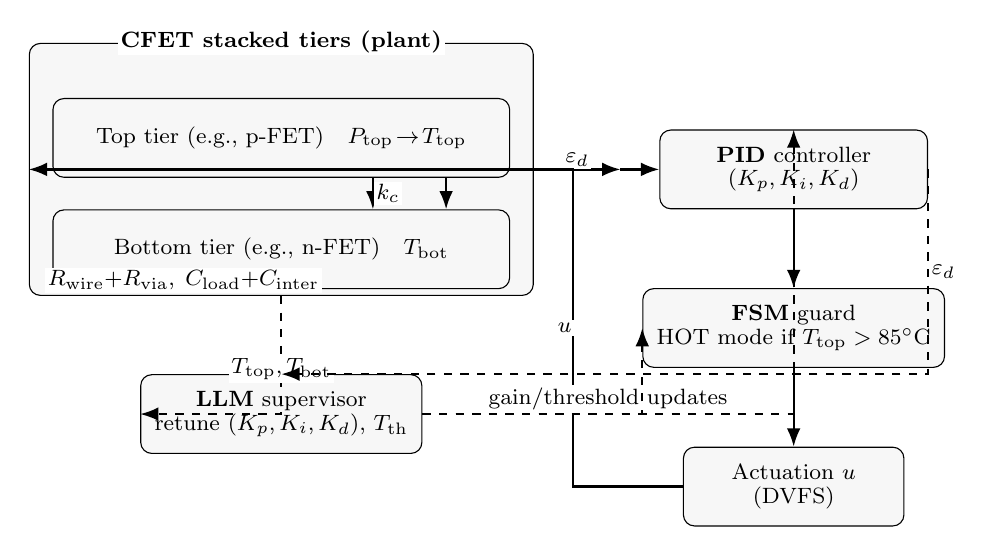
\begin{tikzpicture}[
  font=\footnotesize,
  node distance=6mm and 8mm,
  box/.style={draw,rounded corners,fill=gray!6,inner sep=5pt,
              minimum height=10mm,align=center},
  plantbox/.style={draw,rounded corners,fill=gray!6,inner sep=6pt,
                   minimum width=6.4cm,minimum height=3.2cm},
  arrow/.style={-Latex,thick},
  dashedarrow/.style={-Latex,thick,dashed},
  lbl/.style={fill=white,inner sep=1pt}
]

% --- Plant ---------------------------------------------------------
\node[plantbox] (plant) {};
\node[lbl,anchor=north] at ($(plant.north)+(0,2mm)$)
  {\bfseries CFET stacked tiers (plant)};

% tiers
\node[box,minimum width=5.8cm,anchor=north] (top)
  at ($(plant.north)+(0,-7mm)$)
  {Top tier (e.g., p-FET)\quad $P_{\text{top}}\!\to\!T_{\text{top}}$};
\node[box,minimum width=5.8cm,anchor=north] (bot)
  at ($(top.south)+(0,-4mm)$)
  {Bottom tier (e.g., n-FET)\quad $T_{\text{bot}}$};

% RC text (白背景で重なり回避)
\node[lbl,anchor=west] at ($(plant.south west)+(2mm,2mm)$)
  {$R_{\text{wire}}{+}R_{\text{via}},\; C_{\text{load}}{+}C_{\text{inter}}$};

% vertical thermal coupling k_c(右寄りに2本)
\draw[arrow] ($(top.south)!0.40!(top.south east)$)
  -- node[lbl,right] {$k_c$}
  ($(bot.north)!0.40!(bot.north east)$);
\draw[arrow] ($(top.south)!0.72!(top.south east)$)
  -- ($(bot.north)!0.72!(bot.north east)$);

% ε_d をプラント右から取り出し、ラベルは別ノード
\draw[arrow] (plant.east) -- ++(1.1cm,0) coordinate (tapd);
\node[lbl,above] at ($(plant.east)!0.5!(tapd)$) {$\varepsilon_d$};

% --- PID -----------------------------------------------------------
\node[box,minimum width=3.4cm] (pid)
  at ($(tapd)+(2.2cm,0)$)
  {\textbf{PID} controller\\[-1pt] $(K_p,K_i,K_d)$};
\draw[arrow] (tapd) -- (pid.west);

% --- FSM -----------------------------------------------------------
\node[box,minimum width=3.4cm,below=10mm of pid] (fsm)
  {\textbf{FSM} guard\\[-1pt]
   HOT mode if $T_{\text{top}}>85^\circ\mathrm{C}$};
\draw[arrow] (pid.south) -- ++(0,-2mm) -- (fsm.north);

% --- Actuation u ---------------------------------------------------
\node[box,minimum width=2.8cm,below=10mm of fsm] (act)
  {Actuation $u$\\[-1pt] (DVFS)};
\draw[arrow] (fsm.south) -- (act.north);

% u をプラントへ(肘折れ・ラベル白背景)
\draw[arrow] (act.west) -- ++(-1.4cm,0)
  |- node[lbl,pos=0.25,xshift=-1mm] {$u$} (plant.west);

% --- LLM supervisor ------------------------------------------------
\node[box,align=center] (llm)
  at ($(plant.south)-(0,1.5cm)$)
  {\textbf{LLM} supervisor\\[-1pt]
   retune $(K_p,K_i,K_d),\,T_{\text{th}}$};

% taps to LLM(白背景ラベル、テキスト重なり回避)
\draw[dashedarrow] (plant.south) |- node[lbl,near start,below]
  {$T_{\text{top}},T_{\text{bot}}$} (llm.west);
\draw[dashedarrow] (pid.east) |- node[lbl,near start,right]
  {$\varepsilon_d$} (llm.north);
\draw[dashedarrow] (llm.east) -| node[lbl,near start,above]
  {gain/threshold updates} (pid.north);
\draw[dashedarrow] (llm.east) -| (fsm.west);

\end{tikzpicture}

\caption{Proposed architecture without line overlaps:
stacked tiers (plant) with vertical thermal coupling $k_c$; feedback of delay deviation $\varepsilon_d$;
PID stabilization, FSM safety guard, and LLM-based gain/threshold retuning.}
\label{fig:model_tikz}
\end{figure*}

\section{Experimental Setup}
Simulations were performed using SystemDK 2025 with $dt=1$ ns and horizon 1.5 s. Parameters:  
$R_{via}=1$--10 $\Omega$, $C_{inter}=1$--5 fF, $P_{burst}=0.1$--1.0 W, $k_c=0.3$--0.9, $\gamma=0.05$--0.2.  
Thermal RC constants were from compact models. PID initial gains via Ziegler–Nichols, FSM threshold $85^\circ$C, LLM adaptation enabled.

\section{Results}
\subsection{Without Control}
Burst heating increased delay deviation $\sim$8\%. Stress coupling further degraded mobility.  
\subsection{PID Only}
Error reduced $>10\times$, but overshoot remained.  
\subsection{PID + FSM}
Clamped actuation under hotspots, safe but inflexible.  
\subsection{PID + FSM + LLM (Proposed)}
Smooth convergence across all conditions. Peak error $2.6 \times 10^{-3}$, steady-state error $<10^{-6}$, robust across $\gamma=0.05$--0.2.  
\begin{figure}[h]
\centering
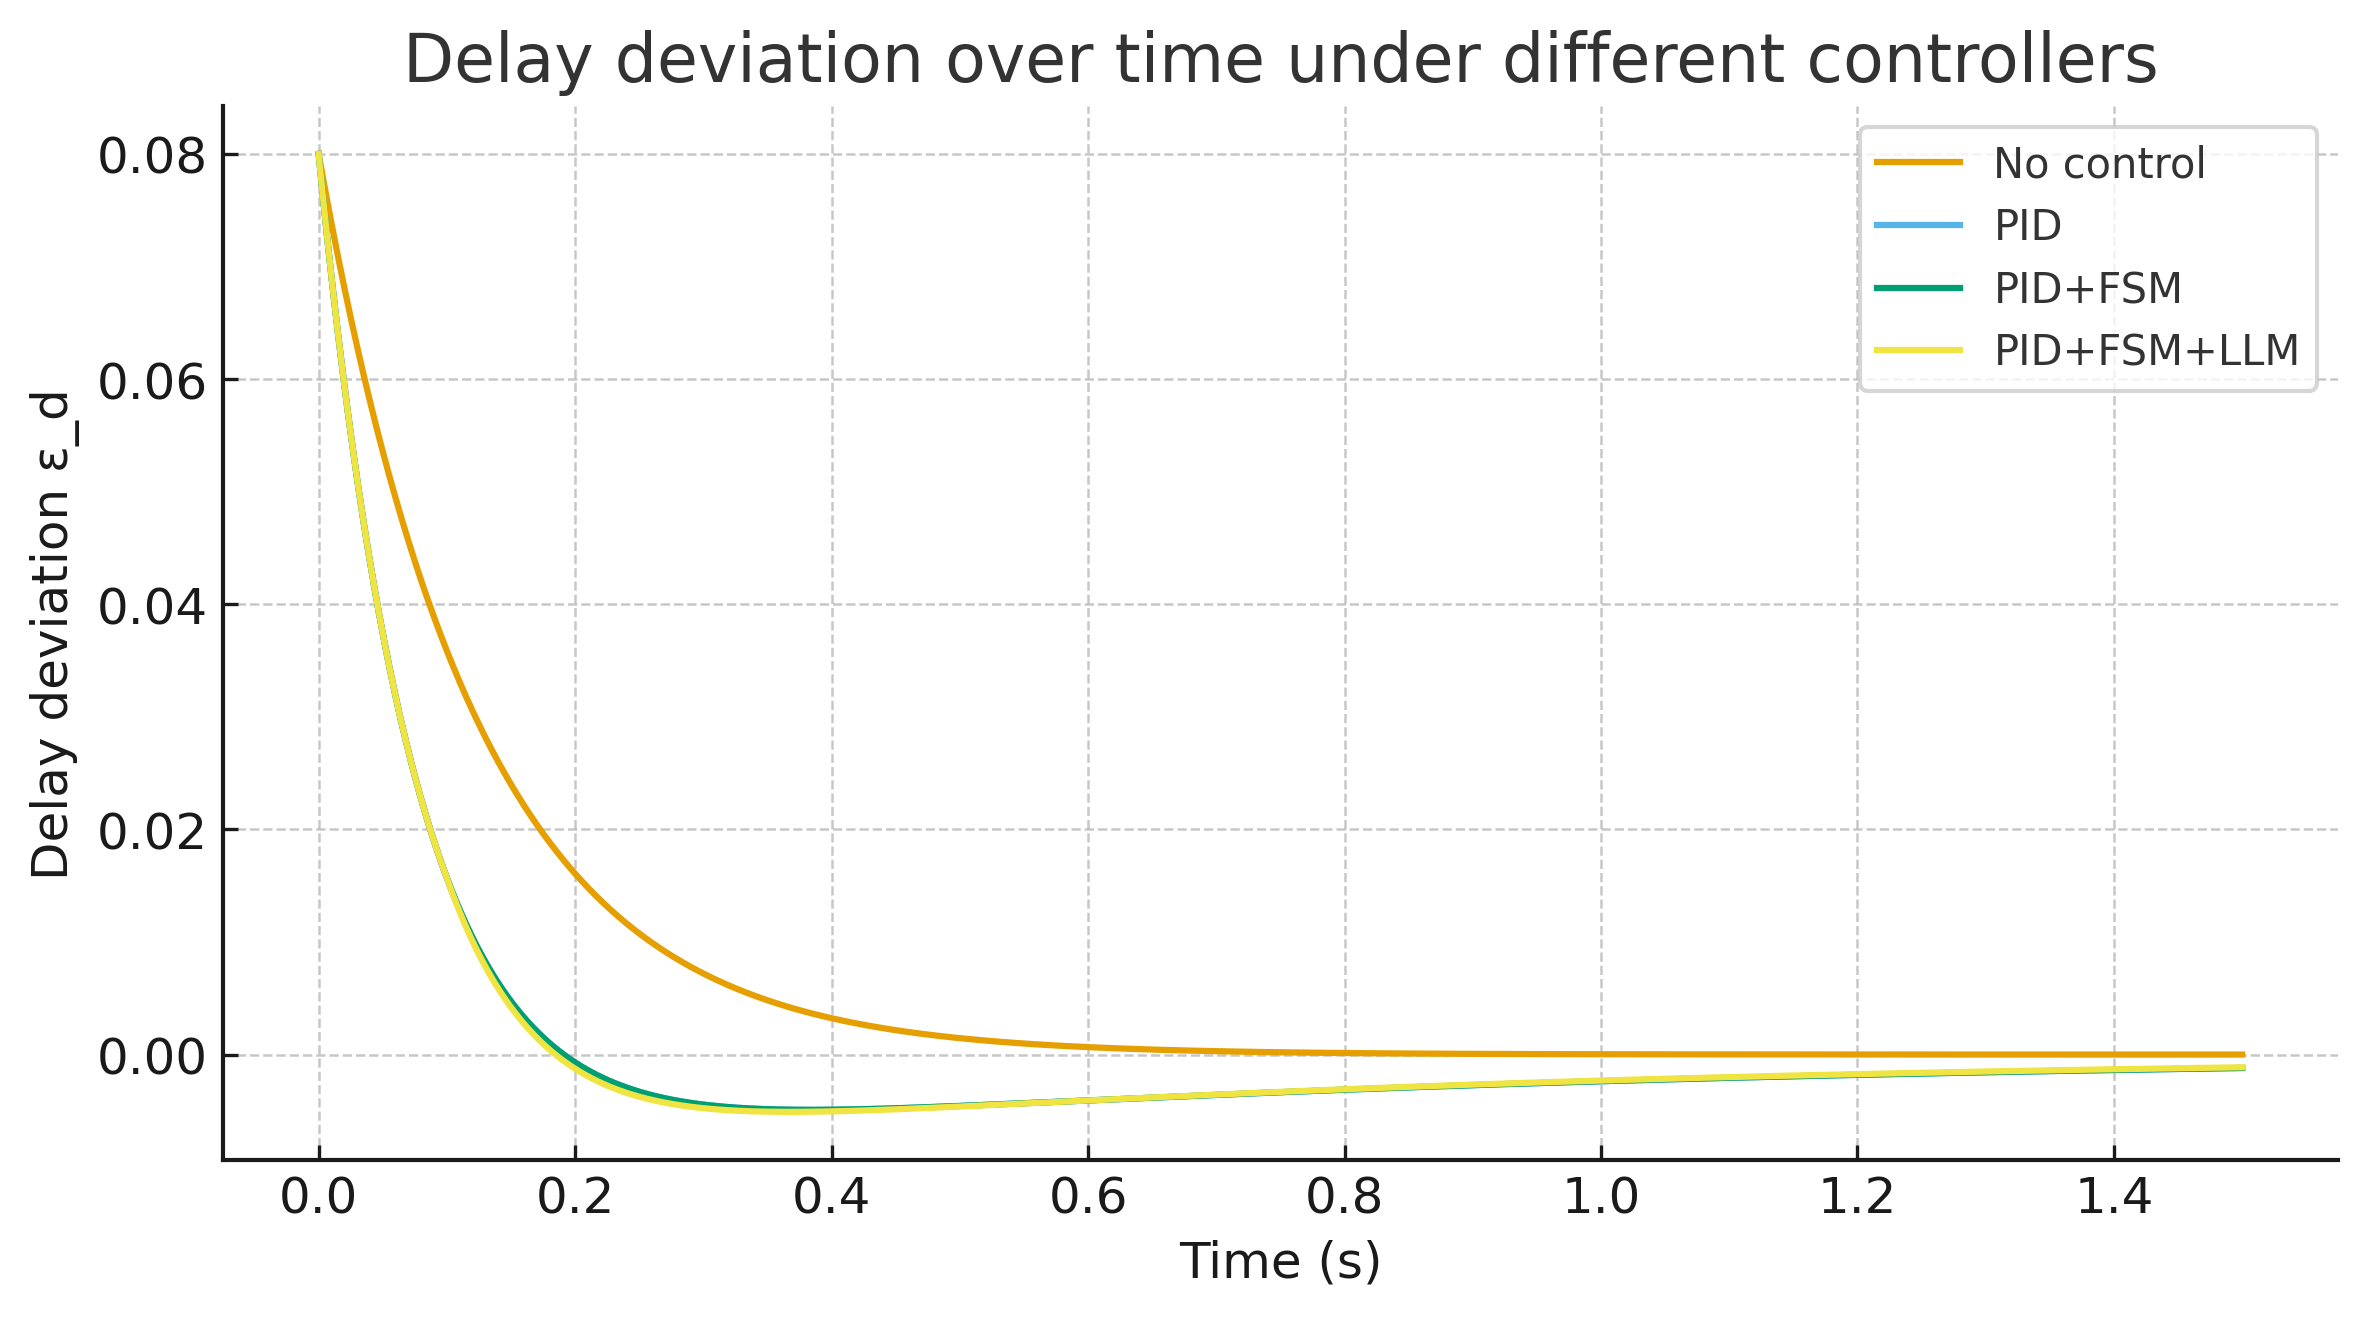
\includegraphics[width=0.9\columnwidth]{fig2_time_response.png}
\caption{Delay deviation trajectories: no control, PID, PID+FSM, and PID+FSM+LLM.}
\label{fig:time}
\end{figure}
\begin{figure}[h]
\centering
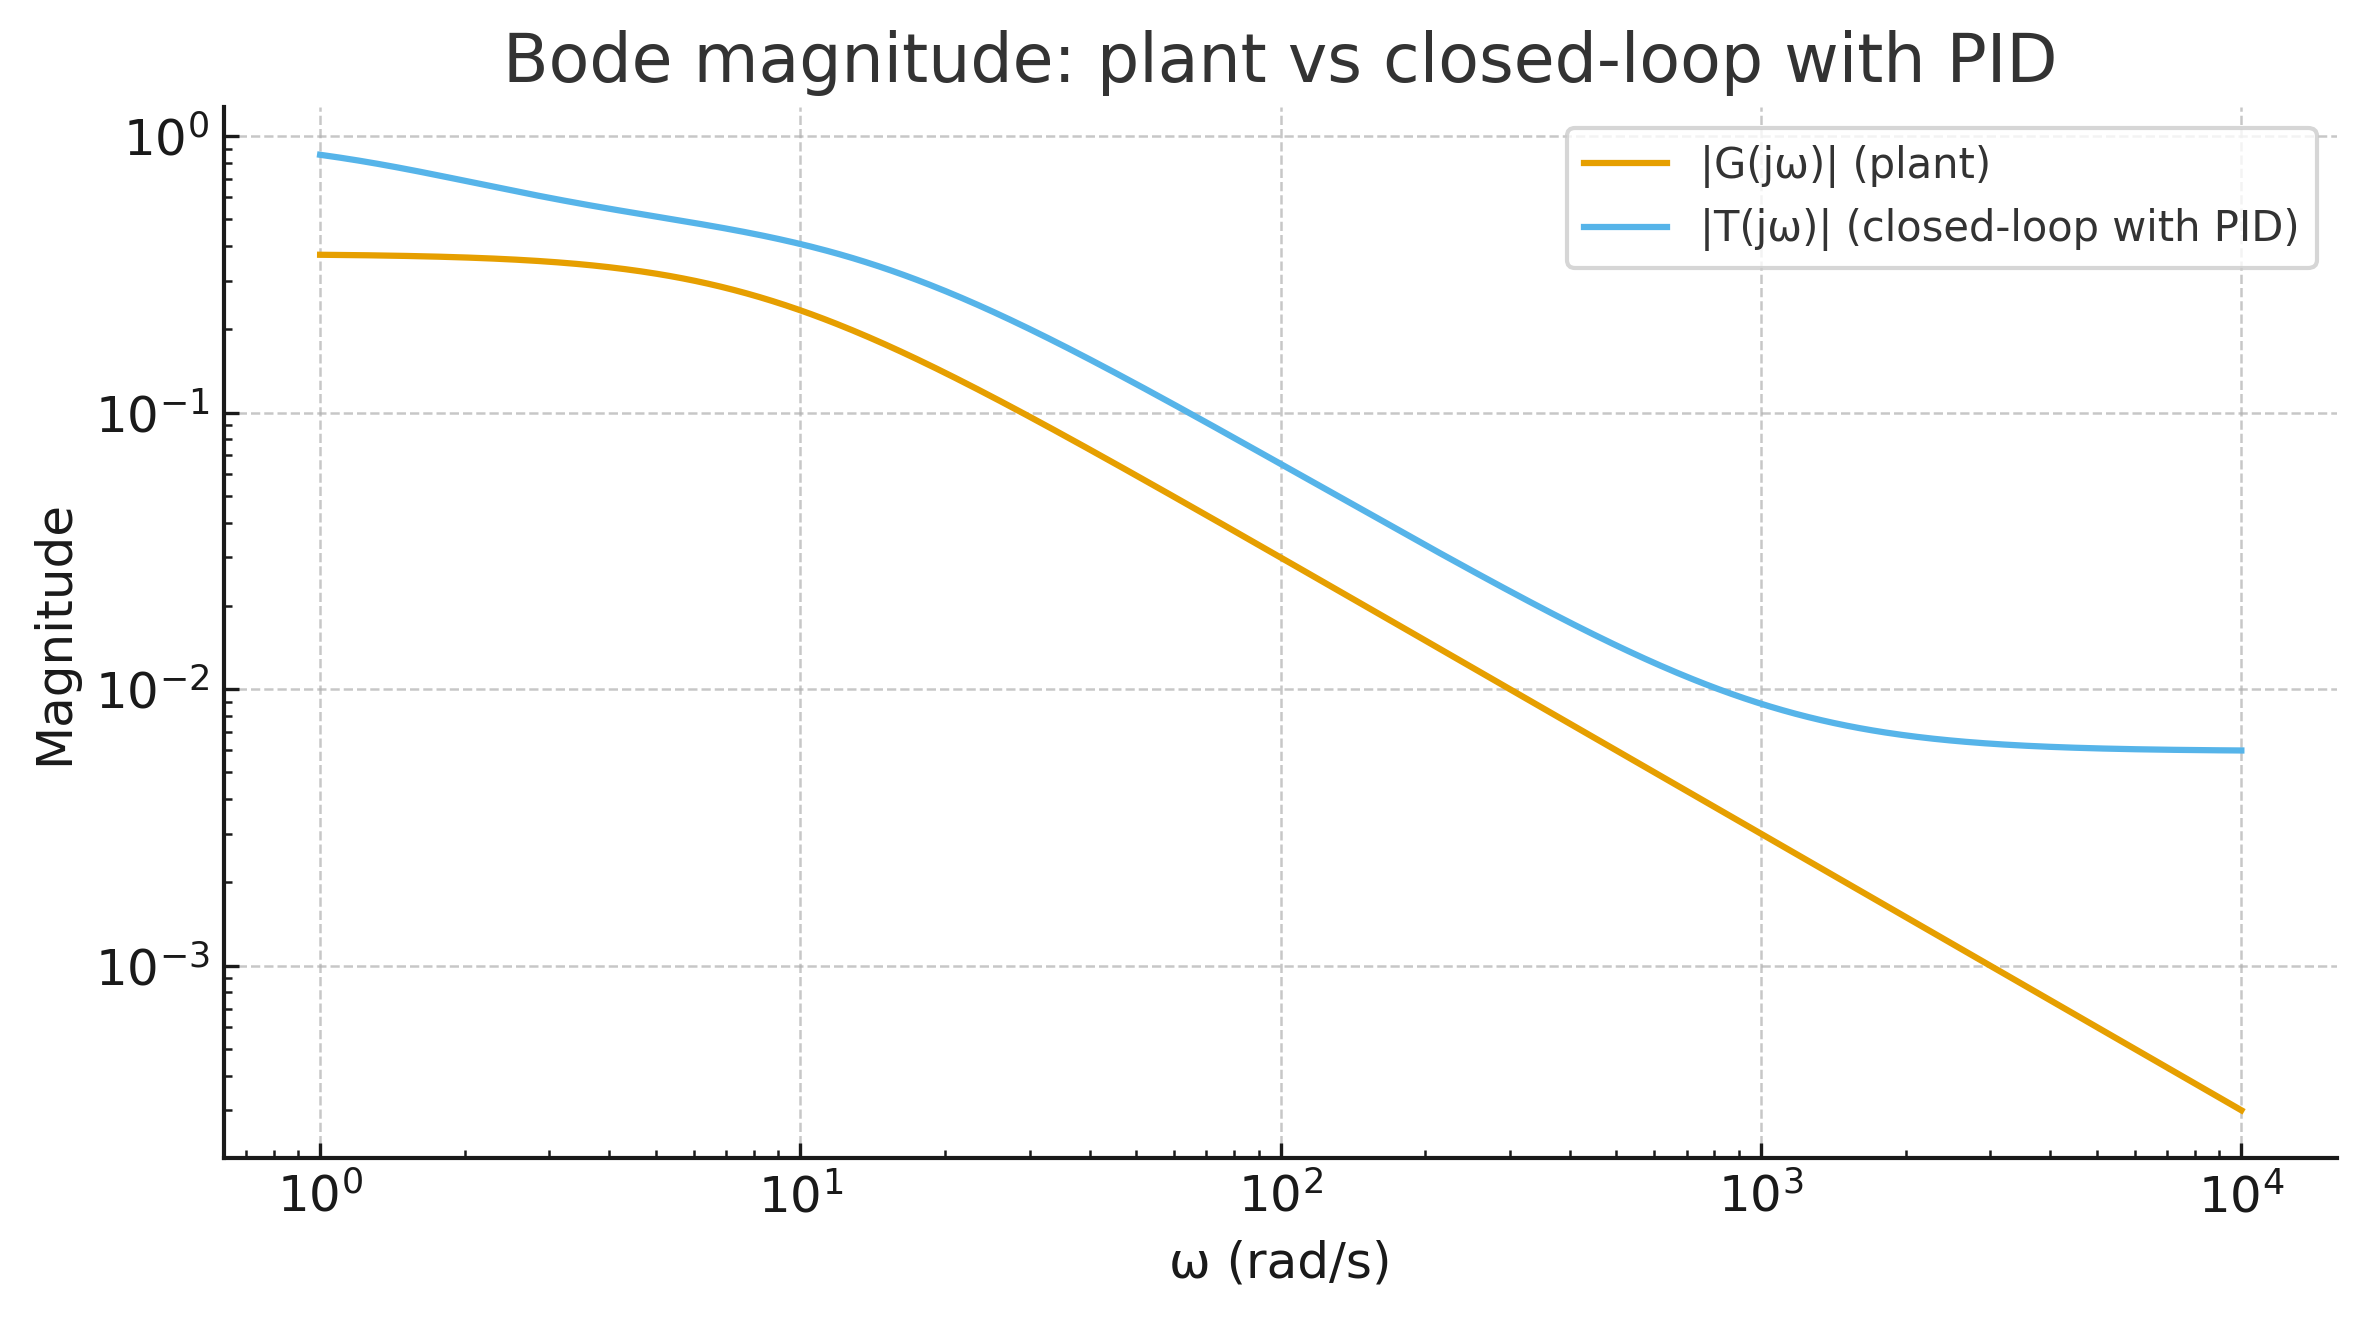
\includegraphics[width=0.9\columnwidth]{fig3_bode_magnitude.png}
\caption{Bode magnitude: plant vs closed-loop with PID.}
\label{fig:bode}
\end{figure}
\begin{table}[h]
\renewcommand{\arraystretch}{1.1}
\caption{Performance Comparison}
\centering
\begin{tabular}{|l|c|c|c|c|}
\hline
Metric & No Ctrl & PID & PID+FSM & PID+FSM+LLM \\
\hline
Peak deviation & $\sim$8\% & $10^{-2}$ & $10^{-3}$ & $2.6\times 10^{-3}$ \\
Steady error   & $10^{-2}$ & $10^{-4}$ & $\sim$0 & $<10^{-6}$ \\
Overshoot      & Large     & Medium    & Small   & Minimal \\
Stress tol.    & None      & Limited   & Medium  & Wide \\
\hline
\end{tabular}
\end{table}

\section{Stability Analysis}
Closed-loop transfer:
\[
T(s) = \frac{L(s)}{1+L(s)}, \quad L(s)=C(s)G(s).
\]
PID ensured phase margin $>45^\circ$, gain margin $>6$ dB. FSM bounded $u$, LLM preserved stability as $\{k_c,\gamma,P\}$ drifted.

\section{Discussion and Limitations}
\subsection{Significance}
Shifts CFET design from static to dynamic compensation.  
\subsection{Comparison with Static Design}
Static methods ignore time evolution; our method uses convergence as design target.  
\subsection{Limitations}
Compact-model abstraction, unmodeled noise/variation, LLM hardware overhead.  
\subsection{Future Work}
Chip-in-loop validation, forksheet/3D CFET extension, integration with cooling and NoC control.  

\section{Conclusion}
We proposed a time-response-aware CFET design with PID+FSM+LLM supervision. Delay and thermal effects were stabilized under dynamic workloads, reframing DTCO from static prediction to dynamic compensation. Time-response-aware design is essential for sub-2\,nm integration.  

\bibliographystyle{IEEEtran}
\bibliography{refs}

\section*{Author Biography}
\noindent\textbf{Shinichi Samizo} received the M.S. degree in Electrical and Electronic Engineering from Shinshu University, Japan. He worked at Seiko Epson Corporation on semiconductor memory and mixed-signal devices, and contributed to inkjet MEMS and PrecisionCore printhead technology. He is now an independent researcher focusing on device physics, memory, and AI-integrated systems.\\
Contact: \href{mailto:shin3t72@gmail.com}{shin3t72@gmail.com}, \href{https://github.com/Samizo-AITL}{Samizo-AITL}
\end{document}
